% Created 2024-08-29 Thu 23:40
% Intended LaTeX compiler: lualatex
\documentclass[bigger]{beamer}
\usepackage{amsmath}
\usepackage{fontspec}
\usepackage{graphicx}
\usepackage{longtable}
\usepackage{wrapfig}
\usepackage{rotating}
\usepackage[normalem]{ulem}
\usepackage{capt-of}
\usepackage{hyperref}
\usetheme[progressbar=foot, sectionpage=none, numbering=fraction]{metropolis}
\usepackage{tikz}
\usepackage{booktabs}
\usepackage{adjustbox}
\usepackage{diagbox}
\usepackage{latexcolors}
\usetikzlibrary{automata, positioning, arrows, arrows.meta}
\usepackage{diagbox}
\usepackage{dsfont}
\usepackage{amsmath}
\usepackage{fontawesome}
\usepackage{pgfgantt}
\usepackage[ruled]{algorithm2e}
\usepackage[absolute, overlay]{textpos}
\definecolor{RedBrown}{RGB}{192, 4, 4} \setbeamercolor{progress bar}{fg=RedBrown} \setbeamercolor{title separator}{fg=RedBrown}
\setbeamercolor{progress bar in head/foot}{fg=RedBrown} \setbeamercolor{progress bar in section page}{fg=RedBrown} \setbeamercolor{alerted text}{fg=RedBrown}
\pretocmd{\tableofcontents}{\thispagestyle{empty}}{}{}
\usepackage{listings}
\usepackage{xcolor}
\definecolor{codegreen}{rgb}{0,0.6,0}
\definecolor{codegray}{rgb}{0.5,0.5,0.5}
\definecolor{codepurple}{rgb}{0.58,0,0.82}
\definecolor{backcolour}{HTML}{f0f0f0}
\lstdefinestyle{mystyle}{
backgroundcolor=\color{backcolour},
commentstyle=\color{codegreen},
keywordstyle=\color{magenta},
numberstyle=\tiny\color{codegray},
stringstyle=\color{codepurple},
basicstyle=\ttfamily,
breakatwhitespace=false,
breaklines=true,
captionpos=b,
keepspaces=true,
numbers=none,
numbersep=5pt,
showspaces=false,
showstringspaces=false,
showtabs=false,
tabsize=2
}
\lstset{style=mystyle}
\usetheme{default}
\author{Andrea Pierré}
\date{August 30, 2024}
\title{Implementation discussion}
\institute{Brown University}
\titlegraphic{\hfill\includegraphics[height=1.5cm]{img/Brown Logo_2016_2 Color Process ST_1300.png}}
\setbeamercovered{transparent=10}
\setbeamertemplate{section in toc}[sections numbered]
\definecolor{headercolor}{HTML}{151b23}
\setbeamercolor{normal text}{%
% bg=,
fg=headercolor
}
\hypersetup{
 pdfauthor={Andrea Pierré},
 pdftitle={Implementation discussion},
 pdfkeywords={},
 pdfsubject={},
 pdfcreator={Emacs 29.4 (Org mode 9.8)}, 
 pdflang={English}}
\begin{document}

\maketitle
\section{Questions}
\label{sec:org4e2530a}
\begin{frame}[label={sec:orgf051d1b}]{Should there be a backward action?}
\begin{center}
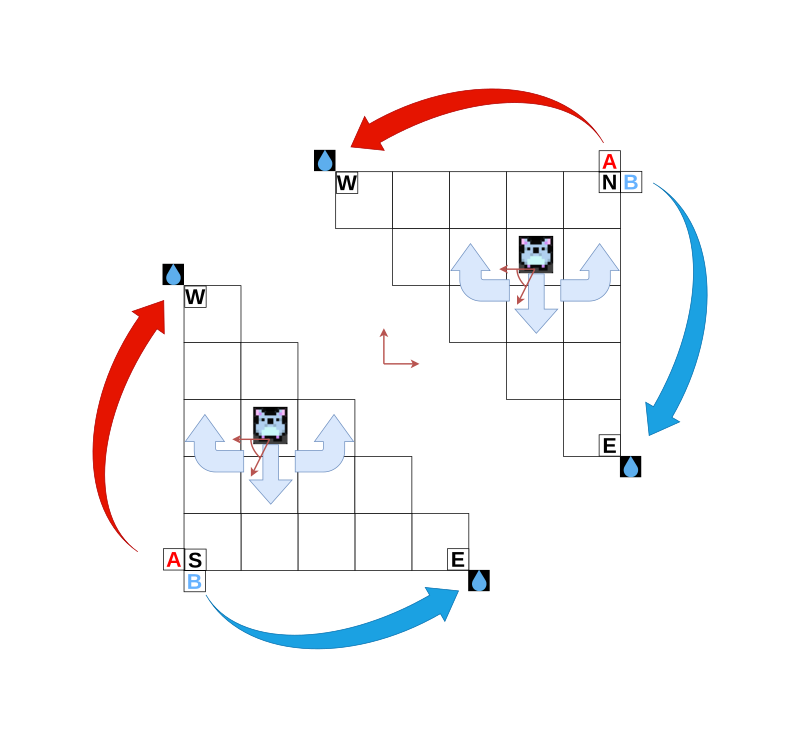
\includegraphics[height=0.8\textheight]{img/RL_env-cartesian-polar.drawio.pdf}
\end{center}
\end{frame}
\begin{frame}[label={sec:orgf3f09f1},fragile]{What should be part of the state?}
\scriptsize
\begin{lstlisting}[language={Python}]
state = TensorDict(
    {
        "cue": torch.tensor(Cues.NoOdor.value, device=DEVICE).unsqueeze(-1),
        "x": torch.tensor([x], device=DEVICE),
        "y": torch.tensor([y], device=DEVICE),
        "direction": torch.tensor([direction], device=DEVICE),
    },
    batch_size=[1],
    device=DEVICE,
)
\end{lstlisting}
\normalsize
\(\to\) Should head direction be part of the state?
\end{frame}
\begin{frame}[label={sec:orgb062178}]{Tiles on the diagonal}
\begin{columns}
\begin{column}[t]{0.6\columnwidth}
\begin{center}
\includegraphics[width=.9\linewidth]{img/policy.png}
\end{center}
\end{column}
\begin{column}[t]{0.4\columnwidth}
\begin{center}
\includegraphics[width=.9\linewidth]{img/task-left-right.jpeg}
\end{center}
\end{column}
\end{columns}
\end{frame}
\begin{frame}[label={sec:org24c9b95}]{Length rounding in polar coordinates?}
\begin{itemize}
\item For step 1 tiles
\item For step 0.5 tiles
\end{itemize}
\begin{center}
\includegraphics[width=.9\linewidth]{img/polar-discretized-length.drawio.pdf}
\end{center}
\end{frame}
\begin{frame}[label={sec:org5241fc7}]{Which architecture for the network?}
\begin{itemize}
\item 2 tasks (East/West \& Left/Right)
\item upper/lower triangle
\item 4 head directions
\item 5 discretized x coordinates (Cartesian)
\item 5 discretized y coordinates (Cartesian)
\item 360 discretized angles (polar)
\item 50 discretized lengths (polar)
\end{itemize}
\end{frame}
\end{document}
